% This file is generated by the MATLAB m-file laprint.m. It can be included
% into LaTeX documents using the packages graphicx, color and psfrag.
% It is accompanied by a postscript file. A sample LaTeX file is:
 \documentclass{article}\usepackage[margin=1cm]{geometry}\usepackage{graphicx,color,psfrag,sfmath}

 \begin{document}
\thispagestyle{plain}
\vspace{2cm}\textsf{
% See http://www.mathworks.de/matlabcentral/fileexchange/loadFile.do?objectId=4638
% for recent versions of laprint.m.
%
% created by:           LaPrint version 3.16 (13.9.2004)
% created on:           16-Oct-2009 14:38:52
% eps bounding box:     37.5 cm x 6.6071 cm
% comment:              
%
\begin{psfrags}%
\psfragscanon%
%
% text strings:
\psfrag{s06}[t][t]{\color[rgb]{0,0,0}\setlength{\tabcolsep}{0pt}\begin{tabular}{c}Cortical Depth from Pia ($\mu m$)\end{tabular}}%
\psfrag{s07}[b][b]{\color[rgb]{1,0,0}\setlength{\tabcolsep}{0pt}\begin{tabular}{c}Glut Synapses per $\mu m^3$\end{tabular}}%
\psfrag{s09}[b][b]{\color[rgb]{0,0,0}\setlength{\tabcolsep}{0pt}\begin{tabular}{c}Cortical Synaptic Density Profile\end{tabular}}%
\psfrag{s11}[][]{\color[rgb]{0,0,0}\setlength{\tabcolsep}{0pt}\begin{tabular}{c} \end{tabular}}%
\psfrag{s12}[][]{\color[rgb]{0,0,0}\setlength{\tabcolsep}{0pt}\begin{tabular}{c} \end{tabular}}%
\psfrag{s15}[t][t]{\color[rgb]{0,0,1}\setlength{\tabcolsep}{0pt}\begin{tabular}{c}GABA Synapses per $\mu m^3$\end{tabular}}%
\psfrag{s18}[l][l]{\color[rgb]{0,0,0}GABA}%
\psfrag{s19}[l][l]{\color[rgb]{0,0,0}Glut}%
\psfrag{s20}[l][l]{\color[rgb]{0,0,0}GABA}%
%
% xticklabels:
\psfrag{x01}[t][t]{0}%
\psfrag{x02}[t][t]{100}%
\psfrag{x03}[t][t]{200}%
\psfrag{x04}[t][t]{300}%
\psfrag{x05}[t][t]{400}%
\psfrag{x06}[t][t]{500}%
\psfrag{x07}[t][t]{600}%
\psfrag{x08}[t][t]{700}%
\psfrag{x09}[t][t]{800}%
\psfrag{x10}[t][t]{900}%
\psfrag{x11}[t][t]{1000}%
\psfrag{x12}[t][t]{0}%
\psfrag{x13}[t][t]{100}%
\psfrag{x14}[t][t]{200}%
\psfrag{x15}[t][t]{300}%
\psfrag{x16}[t][t]{400}%
\psfrag{x17}[t][t]{500}%
\psfrag{x18}[t][t]{600}%
\psfrag{x19}[t][t]{700}%
\psfrag{x20}[t][t]{800}%
\psfrag{x21}[t][t]{900}%
\psfrag{x22}[t][t]{1000}%
%
% yticklabels:
\psfrag{v01}[l][l]{0}%
\psfrag{v02}[l][l]{0.02}%
\psfrag{v03}[l][l]{0.04}%
\psfrag{v04}[l][l]{0.06}%
\psfrag{v05}[l][l]{0.08}%
\psfrag{v06}[r][r]{0.4}%
\psfrag{v07}[r][r]{0.8}%
\psfrag{v08}[r][r]{1.2}%
\psfrag{v09}[r][r]{1.6}%
\psfrag{v10}[r][r]{2}%
%
% Figure:
\resizebox{30cm}{!}{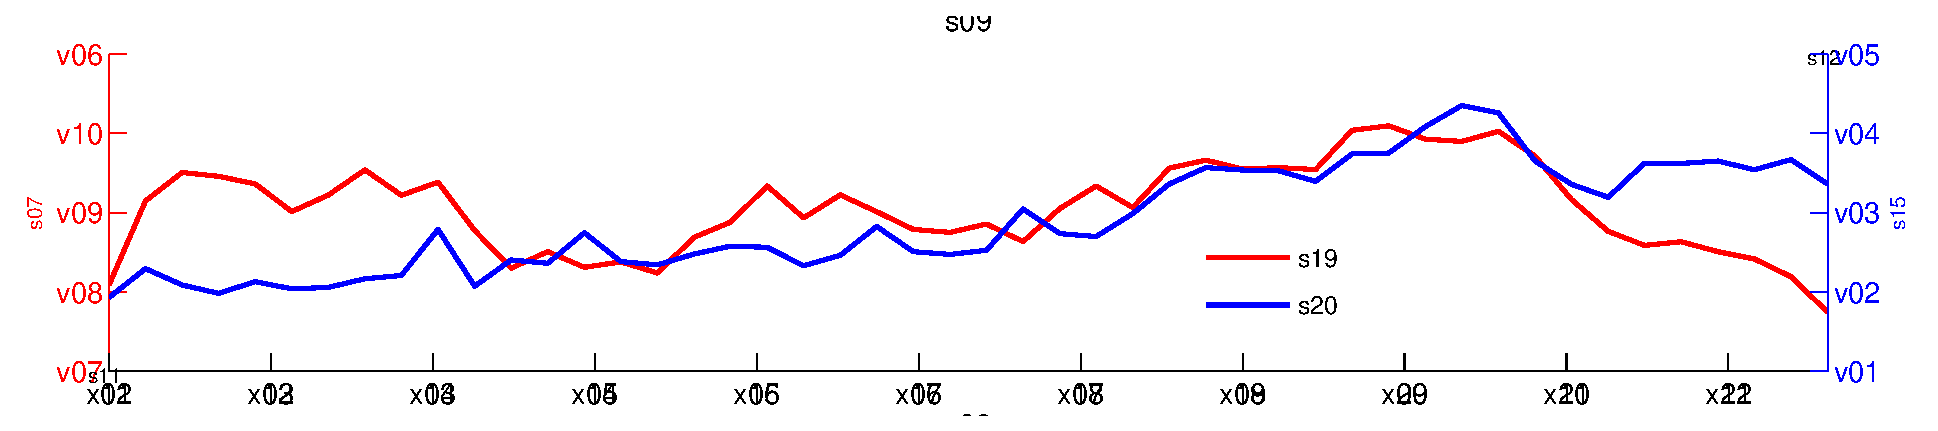
\includegraphics{fig-synprof-wide.eps}}%
\end{psfrags}%
%
}\end{document}
